\section{Numerical results}
LiftedKKT and HyKKT has been implemented on the GPU
We compare the performance of LiftedKKT and HyKKT with HSL on two benchmarks.
First, we detail in \S\ref{sec:num:pprof} the respective performance of the two hybrid solvers
on a large-scale OPF instance. Then, we present in \S\ref{sec:num:opf}
the results we get on the PGLIB OPF benchmark, complemented in \S\ref{sec:num:cops} by
the COPS benchmark.

\subsection{Implementation}

\paragraph{IPM solver.}
We have implemented the two condensed-space methods in our nonlinear IPM solver MadNLP~\cite{shin2021graph}.
This implementation utilizes the abstraction {\tt AbstractKKTSystem} to represent the various formulations of the KKT linear systems.
MadNLP can deport most of the IPM algorithm to the GPU, except for basic IPM operations used for the coordination, such as the filter line-search algorithm.

\paragraph{Evaluation of the nonlinear models.}
We use the ExaModels.jl modeling tool~\cite{shin2023accelerating} to implement all the nonlinear programs utilized in our benchmark.
ExaModels.jl harnesses the implicit sparsity structure and provides custom derivative kernels for repetitive algebraic subexpressions of the constraints and objective functions to compute first and second-order derivatives on the GPU in parallel~\cite{bischof1991exploiting,enzyme2021}.
This approach caters to the SIMD architecture of the GPU by assigning each expression to multiple threads responsible for computing derivatives for different values.

\paragraph{Linear solvers.}
We factorize the KKT systems assembled within MadNLP using various sparse linear solvers, chosen based on the KKT formulation (K1, K2, K3) and the device (CPU, GPU) being utilized.
In particular, we utilize the following solvers:
\begin{itemize}
  \item {\tt HSL MA27}: Implements the \lblt factorization on the CPU.
    It solves the augmented KKT system~\eqref{eq:kkt:augmented}.
    This solver serves as the reference when running on the CPU.
  \item {\tt CHOLMOD}: Implements the Cholesky factorization on the CPU
    (using the AMD ordering \cite{amestoy-david-duff-2004} by default).
    It factorizes the condensed matrix $K_\gamma$ appearing in \eqref{eq:kkt:hykkt}.
    This solver is used to assess the performance of the hybrid solvers when running on the CPU.
  \item {\tt cuDSS}: Implement \llt, \ldlt and \lu decompositions on an NVIDIA GPU.
    We use the Cholesky factorization to factorize the condensed matrix $K_\gamma$ on GPU.
    This newly released solver is the contender in our benchmark.
  \item {\tt Krylov.jl}: Contains the CG method for both CPU and GPU architectures, as part of the Golub \& Greif strategy.
\end{itemize}

We use the Julia language \cite{bezanson-edelman-karpinski-shah-2017} for the comparison, where CHOLMOD \cite{chen-davis-hager-rajamanickam-2008} is included with Julia.
For the HSL linear solvers, we utilize libHSL \cite{fowkes-lister-montoison-orban-2024} with the Julia interface HSL.jl \cite{montoison-orban-hsl-2021}.
HSL MA27 and CHOLMOD are both compiled with OpenBLAS \cite{openblas}, a multithreaded version of BLAS and LAPACK.
The Julia package Krylov.jl~\cite{montoison2023krylov} contains a collection of Krylov methods with a polymorphic implementation that can be used on both CPU and GPU architectures.
% Should we provide the version of the linear solvers?

\subsection{Performance analysis on a large-scale instance}
\label{sec:num:pprof}
We initially evaluate the performance of each KKT solver on a large-scale OPF instance, taken from
the PGLIB benchmark~\cite{babaeinejadsarookolaee2019power}: {\tt 78484epigrids}.
Our formulation with ExaModels has
a total of 674,562 variables, 661,017 equality constraints and 378,045
inequality constraints.
Our previous work has pointed out that as soon as the OPF model is
evaluated on the GPU using ExaModels, the KKT solver is the current bottleneck
in the numerical implementation~\cite{shin2023accelerating}.

\subsubsection{Individual performance of the linear solvers}
Subsequently, we evaluate the individual performance of the cuDSS solver when factorizing the matrix $K_{\gamma}$ at the first IPM iteration (here with $\gamma = 10^7$).
We compare the times to perform the symbolic analysis,
the factorization and the triangular solves with CHOLMOD.

The results are displayed in Table~\ref{tab:linsol:time}.
We benchmark the three decompositions implemented in cuDSS (\llt, \ldlt, \lu), and assess the accuracy of the solution by computing the infinity norm of the residual.
% The accuracy of the solution depends of on more factors than the backsolve.
% The main error comes from the factorization.
We observe that the analysis phase is four times slower for cuDSS compared to CHOLMOD.
Fortunately, this operation only needs to be computed once, meaning that its cost is amortized if we run many IPM iterations.
The factorization is about twenty times faster in cuDSS, with a time almost independent of the algorithm being used.
The backward and forward sweeps are ten times faster.
% The triangular solves don't parallelize well on a GPU.
In terms of accuracy, the quality of the solution remains on par with CHOLMOD, except for the \ldlt decomposition which lags behind by at least two orders of magnitude.

% \begin{table}[!ht]
%   \centering
%   \resizebox{\textwidth}{!}{
%   \begin{tabular}{|lrrrr|}
%   \hline
%   linear solver & analysis (s) & factorization (s) & backsolve (s) & accuracy \\
%   \hline
%     cholmod     & 0.798 &$6.34\times 10^{-1}$&$5.50\times 10^{-2}$&$3.60\times 10^{-13}$\\
%     cudss-\llt  & 3.50  &$4.77\times 10^{-2}$&$2.08\times 10^{-2}$&$2.64\times 10^{-13}$\\
%     cudss-\lu   & 3.48  &$4.97\times 10^{-2}$&$1.91\times 10^{-2}$&$2.58\times 10^{-13}$\\
%     cudss-\ldlt & 3.49  &$5.80\times 10^{-2}$&$1.88\times 10^{-2}$&$5.44\times 10^{-11}$\\
%   \hline
%   \end{tabular}
%   }
%   \caption{Comparing the performance of cuDSS with CHOLMOD.
%     The matrix $K_\gamma$ is symmetric positive definite, with
%     a size $n = 674,562$. The matrix is extremely sparse, with only $7,342,680$ non-zero entries ($0.002$\%).
%     \label{tab:linsol:time}
%     (A30 GPU)
%   }
% \end{table}

\begin{table}[!ht]
  \centering
  \resizebox{\textwidth}{!}{
  \begin{tabular}{|lrrrr|}
  \hline
  linear solver & analysis (s) & factorization (s) & backsolve (s) & accuracy \\
  \hline
    cholmod     & 1.18  & $8.57 \times 10^{-1}$ & $1.27 \times 10^{-1}$ & $3.60\times 10^{-13}$\\
    cudss-\llt  & 4.52  & $3.75 \times 10^{-2}$ & $1.32 \times 10^{-2}$ & $2.64\times 10^{-13}$\\
    cudss-\lu   & 4.50  & $3.72 \times 10^{-2}$ & $1.49 \times 10^{-2}$ & $2.58\times 10^{-13}$\\
    cudss-\ldlt & 4.50  & $4.07 \times 10^{-2}$ & $1.55 \times 10^{-2}$ & $7.62\times 10^{-11}$\\
  \hline
  \end{tabular}
  }
  \caption{Comparing the performance of cuDSS with CHOLMOD.
    The matrix $K_\gamma$ is symmetric positive definite, with
    a size $n = 674,562$. The matrix is extremely sparse, with only $7,342,680$ non-zero entries ($0.002$\%).
    \label{tab:linsol:time}
    (A100 GPU)
  }
\end{table}

\subsubsection{Tuning the Golub \& Greif strategy}
In Figure~\ref{fig:hybrid:gamma} we depict the evolution of the number
of CG iterations and relative accuracy as we increase the parameter $\gamma$
from $10^4$ to $10^8$.

On the algorithmic side, we observe that the higher the regularization $\gamma$,
the faster the CG algorithm: we decrease the total number of iterations
spent in CG by a factor of 10. However, we have to pay a price in term
of accuracy: for $\gamma > 10^8$ the solution returned by the linear solver
is not accurate enough and the IPM algorithm has to proceed to more
primal-dual regularization, leading to an increase in the total number of iterations.

On the numerical side, the table in Figure~\ref{fig:hybrid:gamma} compares
the time spent in the IPM solver on the CPU (using CHOLMOD) and on the GPU
(using the solver {\tt cuDSS}). Overall {\tt cuDSS} is
faster than CHOLMOD, leading to a 4x-8x speed-up in the total IPM solution time.
The assembling of the condensed matrix $K_\gamma$ also parallelizes well
on the GPU, and reduces from $\approx 8s$ on the CPU to $\approx 0.2s$ on the GPU.

\begin{figure}[!ht]
  \centering
  \resizebox{\textwidth}{!}{
  \begin{tabular}{|r|rrrr >{\bfseries}r|rrrr >{\bfseries}r|}
  \hline
  & \multicolumn{5}{c|}{\bf CHOLMOD (CPU)} & \multicolumn{5}{c|}{\bf cuDSS-\ldlt (CUDA)} \\
  \hline
  $\gamma$ & \# it & cond. (s) & CG (s) & linsol (s) & IPM (s) & \# it & cond. (s) & CG (s) & linsol (s) & IPM (s) \\
  \hline
  $10^4$ & 96 & 8.15 & 463.86 & 536.83 & 575.06 & 96 & 0.17 & 113.27 & 114.52 & 124.00 \\
  $10^5$ & 96 & 8.33 & 163.35 & 235.61 & 273.36 & 96 & 0.17 & 53.37 & 54.62 & 64.39 \\
  $10^6$ & 96 & 8.22 & 68.69 & 139.86 & 177.24 & 96 & 0.17 & 14.53 & 15.78 & 25.39 \\
  $10^7$ & 96 & 8.24 & 35.12 & 107.17 & 144.78 & 96 & 0.17 & 7.95 & 9.20 & 18.41 \\
  $10^8$ & 96 & 7.89 & 21.68 & 93.85 & 131.33 & 96 & 0.17 & 5.36 & 6.62 & 15.90 \\
  \hline
  \end{tabular}
  }
  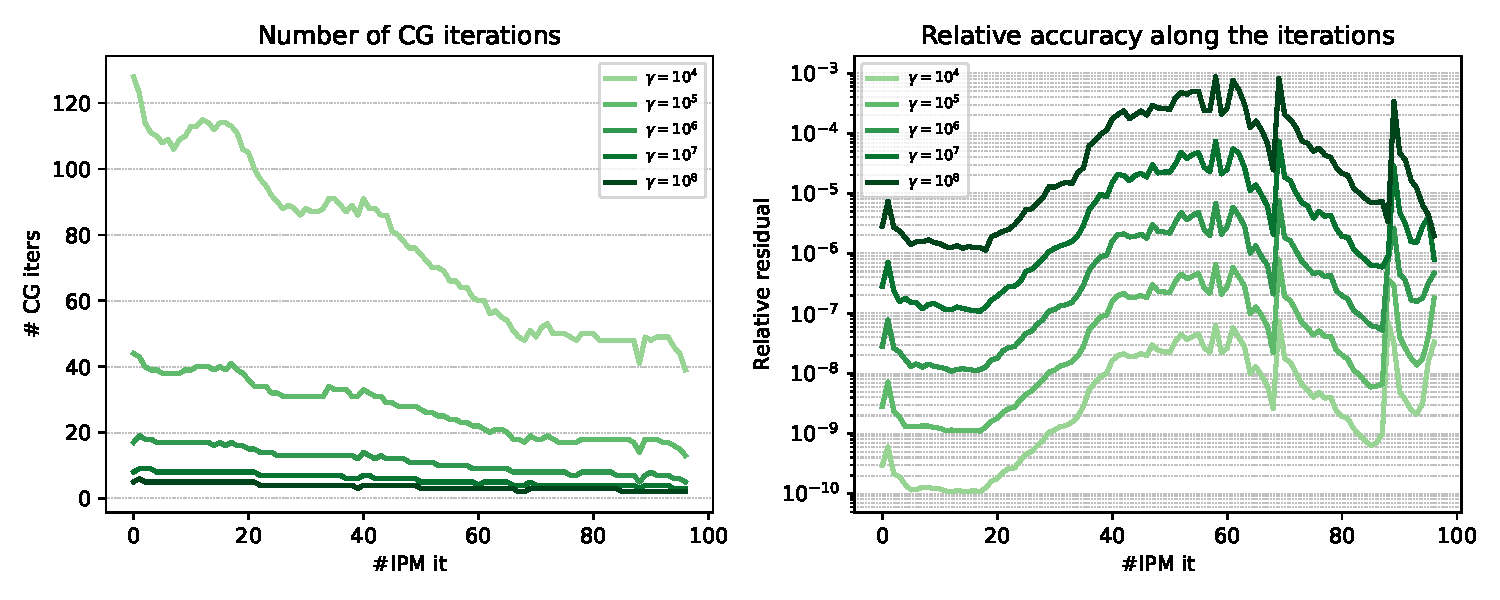
\includegraphics[width=\textwidth]{../figures/hybrid-gamma.pdf}
  \caption{
    Above: Decomposition of IPM solution time across
    (a) condensation time (cond.), (b) CG time, (c) total time
    spent in the linear solver (linsol.) and (d) total time spent in
    IPM solver (IPM).
    Below: Impact of $\gamma$ on the total number of CG iterations
    and the norm of the relative residual at each IPM iteration.
    The peak observed in the norm of the relative residual corresponds
    to the primal-dual regularization performed inside the IPM algorithm,
    applied when the matrix $K_\gamma$ is not positive definite.
    \label{fig:hybrid:gamma}
    (A30 GPU)
  }
\end{figure}


\subsubsection{Tuning the equality relaxation strategy}
We now analyze the numerical performance of LiftedKKT (\S\ref{sec:kkt:sckkt}).
The method solves the KKT system~\eqref{eq:liftedkkt} using a direct solver.
The parameter $\tau$ used in the equality relaxation~\eqref{eq:problemrelaxation}
is set equal to the IPM tolerance $\varepsilon_{tol}$ (in practice, it does not
make sense to set a parameter $\tau$ below IPM tolerance as the
inequality constraints are satisfied only up to a tolerance $\pm \varepsilon_{tol}$
in IPM).

We compare in Table~\ref{tab:sckkt:performance} the performance obtained by LiftedKKT
as we decrease the IPM tolerance $\varepsilon_{tol}$.
We display both the runtimes on the CPU (using CHOLMOD) and on the GPU (using cuDSS).
We observe that LiftedKKT does not converge with CHOLMOD for a tolerance $\varepsilon_{tol} \leq 10^{-5}$.
The slacks associated with the relaxed equality constraints are converging to a value below $2 \tau$,
leading to highly ill-conditioned terms in the diagonal matrices $\Sigma_s$.
As a consequence, the conditioning of the matrix $K_k$ in \eqref{eq:liftedkkt} can increase
above $10^{18}$, leading to a nearly singular linear system. Interestingly,
we can reduce the tolerance $\varepsilon_{tol}$ down to $10^{-8}$ when using {\tt cuDSS}-\ldlt.
We observe {\tt cuDSS} is more stable: the factorization
succeeds, and the loss of accuracy caused by the ill-conditioning is tamed by the multiple
Richardson iterations (reducing the relative accuracy in the residual down to an acceptable level).
As a result, {\tt cuDSS} can solve
the problem to optimality in $\approx 20s$, a time comparable with HyKKT (see Figure~\ref{fig:hybrid:gamma}).

\begin{table}[!ht]
  \centering
  \resizebox{.5\textwidth}{!}{
  \begin{tabular}{|l|rr|rr|}
    \hline
    & \multicolumn{2}{c|}{\bf CHOLMOD (CPU)} & \multicolumn{2}{c|}{\bf cuDSS-\ldlt (CUDA)} \\
    \hline
    $\varepsilon_{tol}$ & \#it & time (s) & \#it & time (s)\\
    \hline
    $10^{-4}$ &151& 358.8& 114 & 19.9\\
    $10^{-5}$ & - & - & 113 & 30.4\\
    $10^{-6}$ & - & - & 109 & 25.0 \\
    $10^{-7}$ & - & - & 104 & 20.1\\
    $10^{-8}$ & - & - & 105 & 20.3 \\
    \hline
  \end{tabular}
  }
  \label{tab:sckkt:performance}
  \caption{Performance of the equality-relaxation
    strategy as we decrease the IPM tolerance $\varepsilon_{tol}$.
    The table displays the wall time on the CPU (using CHOLMOD)
    and on the GPU (using cuDSS-\ldlt). (A30 GPU)
  }
\end{table}

\subsubsection{Breakdown of the time spent in one IPM iteration}
We decompose the time spent in a single
IPM iteration for the available KKT solvers (HSL MA27, LiftedKKT, and HyKKT).
We look at the 5th IPM iteration obtained when solving {\tt 78484epigrids}.
When solving the KKT system, the time can be decomposed into: (1) assembling the
KKT system, (2) factorizing the KKT system, and (3) computing the descent direction with a backsolve.
As depicted in~\ref{fig:timebreakdown}, we observe
that constructing the KKT system represents only a fraction of the computation time, compared
to the factorization and the backsolve. Using {\tt cuDSS}-\ldlt, we observe speedups of
30x and 15x in the factorization compared to MA27 and CHOLMOD running on the CPU.
Once the KKT system is factorized, computing the descent direction with LiftedKKT is faster than with HyKKT
(0.04s compared to 0.13s) as HyKKT has to run a CG algorithm to solve the Schur complement
system~\eqref{eq:kkt:schurcomplhykkt}.

\begin{figure}[!ht]
  \centering
  \resizebox{.7\textwidth}{!}{
    \begin{tabular}{|l|rrrr|}
      \hline
       & build (s) & factorize (s) & backsolve (s) & accuracy \\
      \hline
      hsl        & $3.15\times 10^{-2}$&$1.22 \times 10^{-0} $&$3.58\times 10^{-1}$&$5.52\times 10^{-7}$\\
    sckkt-cpu  & $8.71\times 10^{-2}$&$6.08\times 10^{-1}$&$2.32\times 10^{-1}$&$3.73\times 10^{-9}$\\
    hckkt-cpu  & $7.97\times 10^{-2}$&$6.02\times 10^{-1}$&$7.30\times 10^{-1}$&$3.38\times 10^{-3}$\\
    sckkt-cuda & $2.09\times 10^{-3}$&$4.37\times 10^{-2}$&$3.53\times 10^{-2}$&$4.86\times 10^{-9}$\\
    hckkt-cuda & $1.86\times 10^{-3}$&$3.38\times 10^{-2}$&$1.35\times 10^{-1}$&$3.91\times 10^{-3}$\\
      \hline
    \end{tabular}
  }
  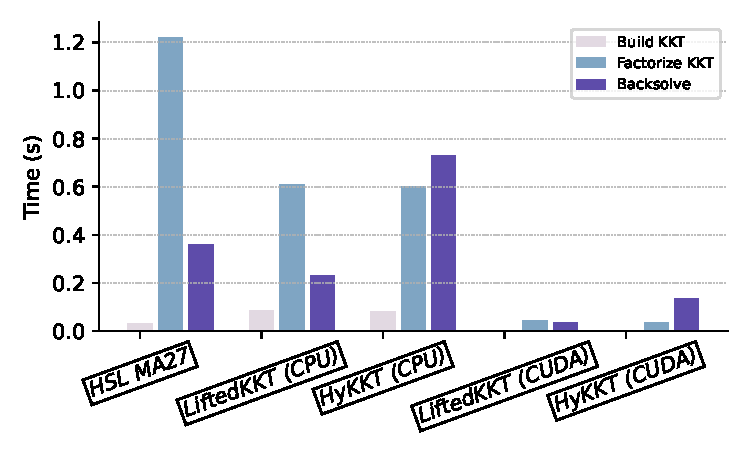
\includegraphics[width=.7\textwidth]{../figures/breakdown.pdf}
  \caption{Breakdown of the time spent in one IPM iteration
    for different linear solvers, when solving {\tt 78484epigrids} (A30 GPU)
  \label{fig:timebreakdown}}
\end{figure}



\subsection{Benchmark on OPF instances}
\label{sec:num:opf}
% The previous subsection has detailed the performance of the two KKT solvers on a specific instance, and highlighted
% the respective downsides of the Golub \& Greif strategy and the equality relaxation strategy.
Now, we run a full benchmark on difficult OPF instances taken
from the PGLIB benchmark~\cite{babaeinejadsarookolaee2019power}.
We compare our two condensed-space methods with HSL MA27 running
on the CPU. The results are displayed in Table~\ref{tab:opf:benchmark}
for an IPM tolerance set to $10^{-4}$.
We complement the table with a Dolan \& Moré performance profile~\cite{dolan2002benchmarking} displayed
in Figure~\ref{fig:opf:pprof}.

Overall, the performance of HSL MA27 is consistent with what was reported
in \cite{babaeinejadsarookolaee2019power}. We observe that HSL MA57 is slower
than HSL MA27 on this particular benchmark, as the OPF instances are super-sparse:
hence, the block elimitation algorithm implemented in HSL MA57 is not beneficial there
\footnote{Personal communication with Iain Duff.}. In addition, we observe that
the automatic differentiation is not the bottleneck in that benchmark, as it contributes to less than 10\% of
the running time on the CPU, and it parallelizes effectively on the GPU when we use ExaModels.

Overall, the equality relaxation strategy gives good results and is faster than
the Golub \& Greif strategy on small and medium instances: indeed, the algorithm
does not have to run a CG algorithm at each IPM iteration, limiting the number
of backsolves to one. However, the method solves only a relaxation of the original
problem, and suffers from the limited accuracy of the equality relaxation strategy:
the algorithm converges in 811 iterations for {\tt 30000\_goc}, leading to a slower
solution time than with HSL ma27.

Regarding HyKKT, we manage to solve all the instances for $\gamma = 10^7$, limiting
the need to tune the parameter $\gamma$ on that particular benchmark. The algorithm
is significantly faster than HSL MA27, but it remains on average slightly slower
than the equality relaxation strategy: the algorithm's weakness is the multiple
backsolves computed at each IPM iteration. For example, compared
to the other instances, the solution of {\tt 8387\_pegase} is impaired
by a larger total number of CG iterations leading to a 4x slowdown compared
to the equality relaxation strategy.
Nevertheless, the performance of HyKKT is better on the largest instances,
with almost an 8x speed-up compared to the reference HSL MA27.

\begin{table}[!ht]
  \centering
  \resizebox{\textwidth}{!}{
		\begin{tabular}{|l|rrr >{\bfseries}r|rrr >{\bfseries}r|rrr >{\bfseries}r|}
			\hline
      & \multicolumn{4}{c|}{\bf HSL MA27} &
			\multicolumn{4}{c|}{\bf LiftedKKT+cuDSS} &
			\multicolumn{4}{c|}{\bf HyKKT+cuDSS} \\
			\hline
			Case & it & AD & lin & total & it & AD & lin & total & it & AD & lin & total \\
			\hline
89\_pegase & 30 & 0.00 & 0.02 & 0.03 & 28 & 0.02 & 0.03 & 0.13 & 30 & 0.03 & 0.06 & 0.17 \\
179\_goc & 43 & 0.00 & 0.03 & 0.05 & 30 & 0.02 & 0.04 & 0.14 & 43 & 0.03 & 0.06 & 0.20 \\
500\_goc & 35 & 0.01 & 0.08 & 0.12 & 36 & 0.02 & 0.04 & 0.19 & 35 & 0.03 & 0.06 & 0.20 \\
793\_goc & 31 & 0.01 & 0.10 & 0.15 & 33 & 0.02 & 0.05 & 0.20 & 31 & 0.03 & 0.08 & 0.23 \\
1354\_pegase & 42 & 0.03 & 0.29 & 0.42 & 44 & 0.04 & 0.08 & 0.32 & 42 & 0.04 & 0.14 & 0.39 \\
			\hline
2000\_goc & 38 & 0.05 & 0.57 & 0.79 & 36 & 0.03 & 0.07 & 0.31 & 38 & 0.03 & 0.13 & 0.42 \\
2312\_goc & 38 & 0.05 & 0.50 & 0.69 & 38 & 0.03 & 0.10 & 0.35 & 38 & 0.03 & 0.18 & 0.46 \\
2742\_goc & 121 & 0.27 & 3.52 & 5.22 & - & - & - & - & - & - & - & - \\
2869\_pegase & 51 & 0.10 & 0.97 & 1.34 & 52 & 0.04 & 0.14 & 0.50 & 51 & 0.05 & 0.26 & 0.65 \\
3022\_goc & 47 & 0.08 & 0.80 & 1.11 & 43 & 0.03 & 0.12 & 0.44 & 47 & 0.04 & 0.19 & 0.54 \\
			\hline
3970\_goc & 44 & 0.12 & 1.71 & 2.35 & 44 & 0.04 & 0.14 & 0.57 & 44 & 0.04 & 0.23 & 0.70 \\
4020\_goc & 57 & 0.17 & 3.62 & 4.41 & 68 & 0.06 & 0.36 & 1.00 & 57 & 0.06 & 0.41 & 1.02 \\
4601\_goc & 66 & 0.20 & 2.79 & 3.70 & 71 & 0.06 & 0.22 & 0.82 & 66 & 0.06 & 0.38 & 1.01 \\
4619\_goc & 46 & 0.16 & 2.90 & 3.67 & 54 & 0.04 & 0.20 & 0.77 & 46 & 0.05 & 0.32 & 0.89 \\
4837\_goc & 55 & 0.18 & 2.26 & 3.12 & 57 & 0.05 & 0.33 & 0.89 & 55 & 0.05 & 0.37 & 0.93 \\
			\hline
4917\_goc & 55 & 0.16 & 1.67 & 2.45 & 48 & 0.04 & 0.19 & 0.64 & 55 & 0.05 & 0.30 & 0.80 \\
5658\_epigrids & 46 & 0.18 & 2.45 & 3.35 & 50 & 0.05 & 0.28 & 0.86 & 46 & 0.05 & 0.35 & 0.94 \\
7336\_epigrids & 45 & 0.22 & 3.13 & 4.18 & 46 & 0.05 & 0.30 & 1.00 & 45 & 0.05 & 0.38 & 1.07 \\
8387\_pegase & 70 & 0.44 & 4.99 & 7.07 & 67 & 0.08 & 0.82 & 1.93 & 70 & 0.08 & 6.86 & 7.97 \\
9241\_pegase & 62 & 0.44 & 5.22 & 7.23 & 63 & 0.08 & 0.73 & 1.86 & 62 & 0.07 & 1.14 & 2.27 \\
			\hline
9591\_goc & 64 & 0.45 & 10.40 & 12.31 & 69 & 0.07 & 0.60 & 1.78 & 64 & 0.08 & 0.87 & 2.03 \\
10000\_goc & 75 & 0.44 & 5.26 & 7.31 & 56 & 0.08 & 0.30 & 1.10 & 75 & 0.09 & 0.86 & 1.88 \\
10192\_epigrids & 50 & 0.42 & 6.94 & 8.80 & 52 & 0.08 & 0.46 & 1.55 & 50 & 0.08 & 0.79 & 1.87 \\
10480\_goc & 65 & 0.54 & 10.71 & 13.15 & 71 & 0.09 & 0.93 & 2.37 & 65 & 0.08 & 1.21 & 2.57 \\
13659\_pegase & 57 & 0.55 & 6.28 & 8.77 & 65 & 0.09 & 1.70 & 3.17 & 57 & 0.07 & 1.16 & 2.64 \\
			\hline
19402\_goc & 70 & 1.20 & 31.11 & 35.93 & 108 & 0.18 & 4.95 & 8.37 & 70 & 0.12 & 2.38 & 4.84 \\
20758\_epigrids & 46 & 0.80 & 12.36 & 15.83 & 2838 & 4.63 & 325.55 & 407.69 & 46 & 0.08 & 1.83 & 3.65 \\
30000\_goc & 130 & 2.66 & 37.02 & 45.88 & 158 & 0.34 & 5.56 & 9.19 & 130 & 0.24 & 4.05 & 7.23 \\
78484\_epigrids & 96 & 7.17 & 166.35 & 192.70 & 128 & 0.48 & 15.97 & 27.49 & 96 & 0.41 & 9.75 & 19.58 \\
			\hline
		\end{tabular}
  }
  \caption{OPF benchmark \label{tab:opf:benchmark}, solved with a tolerance {\tt tol=1e-4}. (A30 GPU)}
\end{table}

\begin{figure}[!ht]
  \centering
  \begin{tabular}{cc}
    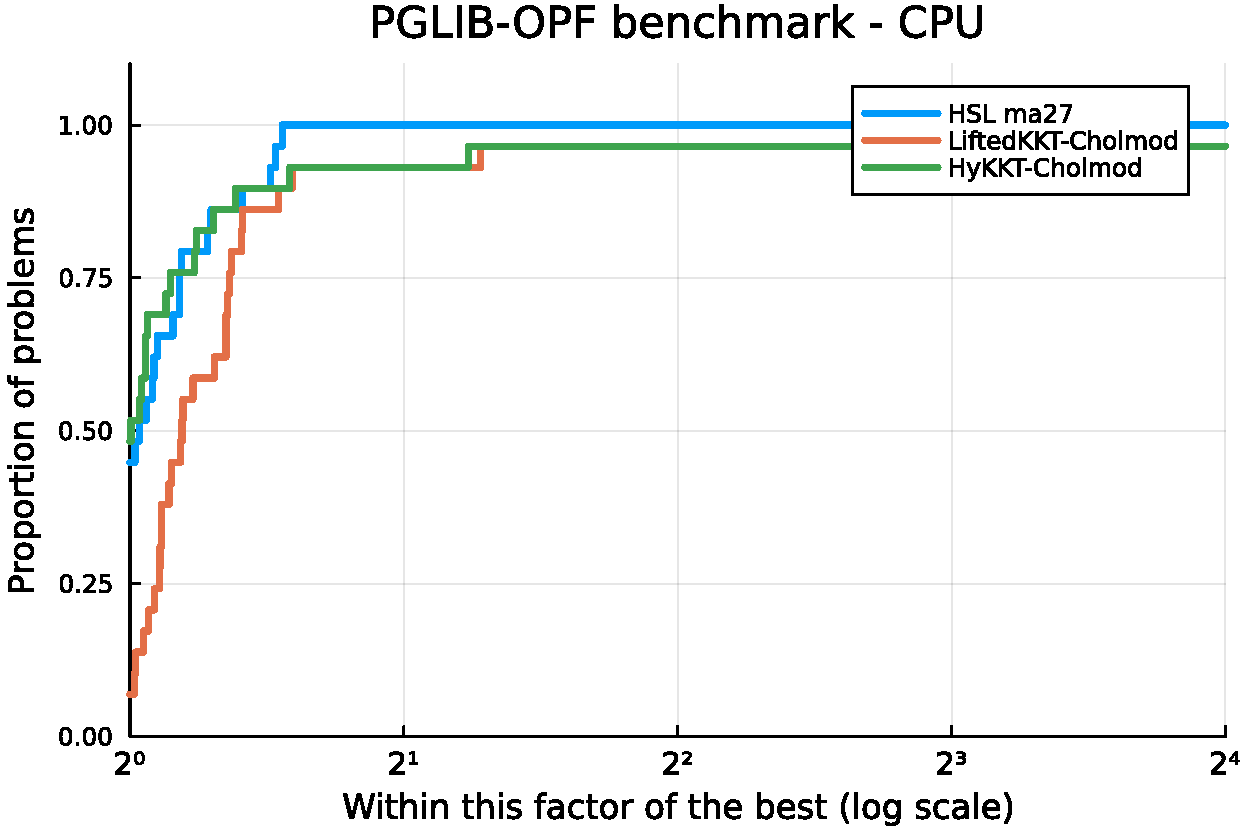
\includegraphics[width=.4\textwidth]{../figures/pprof-cpu.pdf} &
    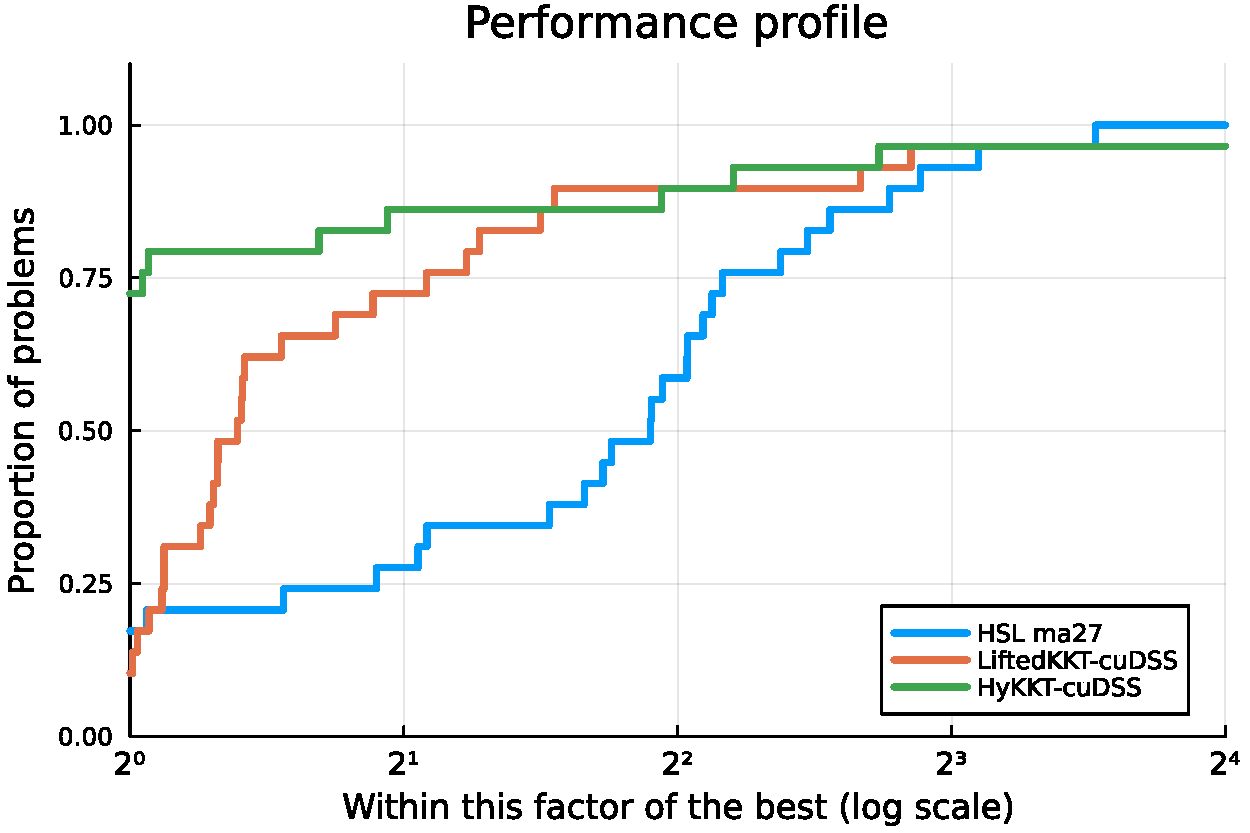
\includegraphics[width=.4\textwidth]{../figures/pprof-cuda.pdf}
  \end{tabular}
  \caption{Performance profile for the PGLIB OPF benchmark, solved
    with a tolerance {\tt tol=1e-4}.
  \label{fig:opf:pprof}}
\end{figure}


\subsection{Benchmark on COPS instances}
\label{sec:num:cops}
We have observed in the previous section that both the equality relaxation
and the HyKKT algorithm gives significant speed-up for large-scale
OPF instances, compared to HSL MA27.
However, the OPF instances are specific nonlinear problems.
For that reason, we have analyzed further the performance of
the equality relaxation and the HyKKT strategies on the COPS benchmark,
which gathers generic nonlinear programs~\cite{dolan2004benchmarking}.
In this section, we look at the performance we get on the particular COPS instances used in
the Mittelmann benchmark, widely used to benchmark nonlinear optimization
solvers~\cite{mittelmann2002benchmark}.
To illustrate the heterogeneity of the COPS instances compared to the
previous OPF problems, we display in Figure~\ref{fig:cops:nnz} the sparsity pattern of the
condensed matrices $K_\gamma$ \eqref{eq:kkt:hykkt} for one OPF instance and for multiple
COPS instances. We observe that some instances ({\tt bearing}) have a sparsity pattern
similar to the OPF instance on the left, whereas some are fully dense ({\tt elec}).
On the opposite, the optimal control instances ({\tt marine}, {\tt pinene}) are
highly sparse and have highly structured Cholesky lower triangular factors.
The results of the COPS benchmark are displayed in Table~\ref{tab:cops:benchmark}.

As expected, the results are different than the previous OPF benchmark.
We observe that HyKKT+cuDSS and SCKKT+cuDSS outperform HSL MA27 on the dense instance {\tt elec}
(25x speed-up) and {\tt bearing} (6x speed-up) --- an instance whose sparsity pattern
is closed to the OPF. In the other instances, both HyKKT+cuDSS and SCKKT+cuDSS are
on par with HSL ma27 and sometimes even slightly slower ({\tt steering}).
In addition, the two solvers HyKKT+cholmod and SCKKT+cholmod offer approximatively
the same performance as HyKKT+cuDSS and SCKKT+cuDSS, respectively, indicating that these
particular instances are less amenable to GPU acceleration.

\begin{figure}[!ht]
  \centering
  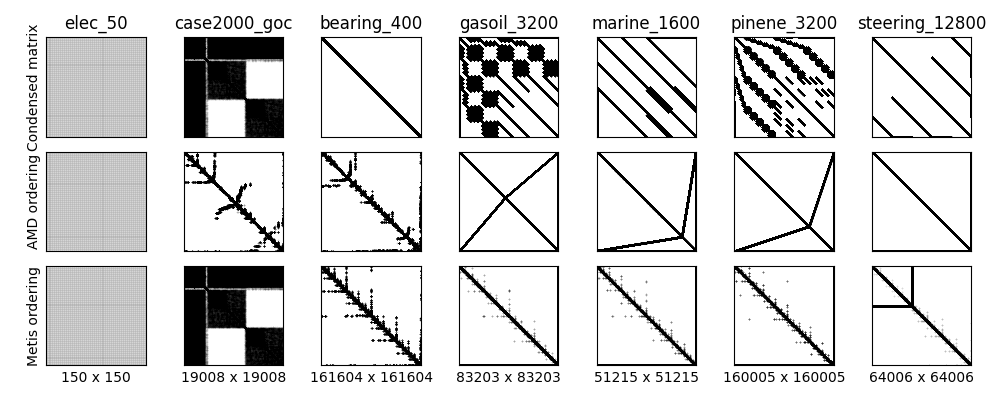
\includegraphics[width=.9\textwidth]{../figures/sparsity_pattern.png}
  \caption{Sparsity patterns for one OPF instance and for various
    COPS problems. The first row displays the sparsity pattern
    of $K_\gamma$, after AMD reordering. The second row displays
    the sparsity pattern of the triangular factor computed by CHOLMOD.
    \label{fig:cops:nnz}
  }
\end{figure}


\begin{table}[!ht]
  \centering
  \resizebox{\textwidth}{!}{
    \begin{tabular}{|l|rr >{\bfseries}r|rr >{\bfseries}r|rr >{\bfseries}r|rr >{\bfseries}r|rr >{\bfseries}r|}
    \hline
    & \multicolumn{3}{c|}{\bf Augmented KKT} &
			\multicolumn{6}{c|}{\bf LiftedKKT} &
			\multicolumn{6}{c|}{\bf HyKKT} \\
      \hline
    & \multicolumn{3}{c|}{\bf HSL MA57} &
			\multicolumn{3}{c|}{\bf CHOLMOD} &
			\multicolumn{3}{c|}{\bf cuDSS+\ldlt} &
			\multicolumn{3}{c|}{\bf CHOLMOD} &
			\multicolumn{3}{c|}{\bf cuDSS+\ldlt} \\
    \hline
      & it & lin & total & it & lin & total & it & lin & total & it & lin & total & it & lin & total \\
    \hline
      bearing\_400 & 17 & 3.33 & 3.95 & 14 & 2.04 & 2.41 & 14 & 0.08 & 0.91 & 14 & 4.94 & 5.42 & 14 & 0.96 & 1.84 \\
      camshape\_6400 & 38 & 0.17 & 0.28 & 35 & 0.04 & 0.38 & 35 & 0.03 & 0.15 & 38 & 0.06 & 0.17 & 38 & 0.03 & 0.20 \\
      elec\_400 & 185 & 23.67 & 32.12 & 139 & 14.70 & 19.42 & 108 & 3.47 & 5.90 & 103 & 9.24 & 12.29 & 104 & 0.59 & 3.66 \\
      gasoil\_3200 & 37 & 4.65 & 5.50 & 20 & 1.76 & 2.41 & 21 & 0.49 & 1.69 & 20 & 1.21 & 1.96 & 20 & 0.32 & 1.33 \\
      marine\_1600 & 13 & 0.39 & 0.47 & 26 & 1.45 & 1.77 & 25 & 0.45 & 1.02 & 13 & 0.33 & 0.49 & 13 & 0.14 & 0.57 \\
      pinene\_3200 & 12 & 1.27 & 1.77 & 21 & 1.58 & 2.83 & 21 & 0.23 & 1.53 & 12 & 3.08 & 3.73 & 11 & 1.38 & 2.48 \\
      robot\_1600 & 55 & 0.65 & 0.77 & 61 & 0.78 & 1.18 & 61 & 0.41 & 1.61 & 34 & 0.24 & 0.44 & 34 & 0.09 & 0.77 \\
      rocket\_12800 & 51 & 3.02 & 4.07 & 37 & 0.62 & 1.69 & 37 & 0.07 & 2.04 & 24 & 1.49 & 2.13 & 24 & 0.41 & 1.89 \\
      steering\_12800 & 19 & 1.44 & 1.81 & 17 & 0.37 & 0.98 & 17 & 0.21 & 1.63 & 22 & 0.63 & 1.01 & 19 & 0.11 & 1.93 \\
    \hline
      bearing\_800 & 13 & 14.12 & 16.04 & 14 & 10.03 & 11.99 & 14 & 0.24 & 3.70 & 12 & 18.76 & 20.60 & 12 & 2.69 & 6.17 \\
      camshape\_12800 & 34 & 0.33 & 0.51 & 33 & 0.08 & 0.26 & 33 & 0.03 & 0.17 & 34 & 0.07 & 0.29 & 34 & 0.04 & 0.23 \\
      elec\_800 & 354 & 325.95 & 396.00 & 212 & 113.83 & 140.31 & 500 & 36.23 & 69.92 & 271 & 149.28 & 179.49 & 272 & 3.77 & 34.77 \\
      gasoil\_12800 & 20 & 11.30 & 13.84 & 25 & 13.86 & 17.02 & 21 & 1.67 & 6.26 & 22 & 6.86 & 9.41 & 22 & 1.89 & 6.28 \\
      marine\_12800 & 11 & 3.41 & 4.54 & 120 & 100.39 & 112.21 & 200 & 51.23 & 75.09 & 11 & 3.77 & 5.03 & 11 & 1.02 & 4.24 \\
      pinene\_12800 & 10 & 6.99 & 8.20 & 21 & 8.76 & 13.35 & 21 & 1.44 & 7.25 & 11 & 12.45 & 15.25 & 12 & 5.31 & 10.23 \\
      robot\_12800 & 35 & 4.44 & 5.92 & 33 & 2.03 & 3.30 & 33 & 0.36 & 4.53 & 35 & 2.00 & 3.26 & 35 & 0.41 & 4.91 \\
      rocket\_51200 & 31 & 6.07 & 9.31 & 38 & 2.83 & 6.78 & 38 & 0.45 & 9.71 & 47 & 14.77 & 21.82 & 31 & 4.10 & 12.33 \\
      steering\_51200 & 27 & 9.47 & 12.67 & 15 & 1.31 & 2.66 & 15 & 0.23 & 5.76 & 23 & 2.65 & 4.47 & 20 & 0.64 & 8.82 \\
    \hline
    \end{tabular}
  }
  \caption{COPS benchmark , solved with a tolerance {\tt tol=1e-6}\label{tab:cops:benchmark} (A30 GPU)}
\end{table}


%%% Local Variables:
%%% mode: latex
%%% TeX-master: "../main"
%%% End:
